\chapter{LFO}
\label{ch:LFO}

\section{Allgemeines}
Wie bereits in Kapitel \label{ch:concept} beschrieben, wird der LFO genutzt, um niederfrequente Signale zu erzeugen. 
Diese Signale werden typischerweise zur Steuerung von nachgelagerten Modulen, wie etwa dem LFO (siehe Kapitel \ref{ch:VCO}), verwendet.
Hierdurch kann beispielsweise die Frequenz des VCO angepasst werden. 
Neben der Frequenz, die der LFO ausgibt, ist auch die entsprechende Signalform für den Klang entscheidend. Hier sind beispielsweise Signalformen, wie Dreieck oder Rechteck möglich.

\section{Schaltplan}
Im Folgenden wird näher auf den Schaltplan des LFO eingegangen, welcher in Abbildung \ref{fig:LFO_Stromlaufplan} zu sehen ist. 
Ein Bauteil von zentraler Bedeutung ist hierbei der Vierfach-Operationsverstärker TL074P. In der gezeigten Schaltung wird dieser als Integrator, Schmitt Trigger, Buffer und LED-Treiber verwendet.
Die grundlegende Funktionsweise dieser Funktionsgruppen wurde bereits in Abschnitt \ref{sec:AnalogePrinzipien} erläutert und wird deshalb nicht erneut aufgezeigt.

\newpage
\begin{figure}[h]
\centering
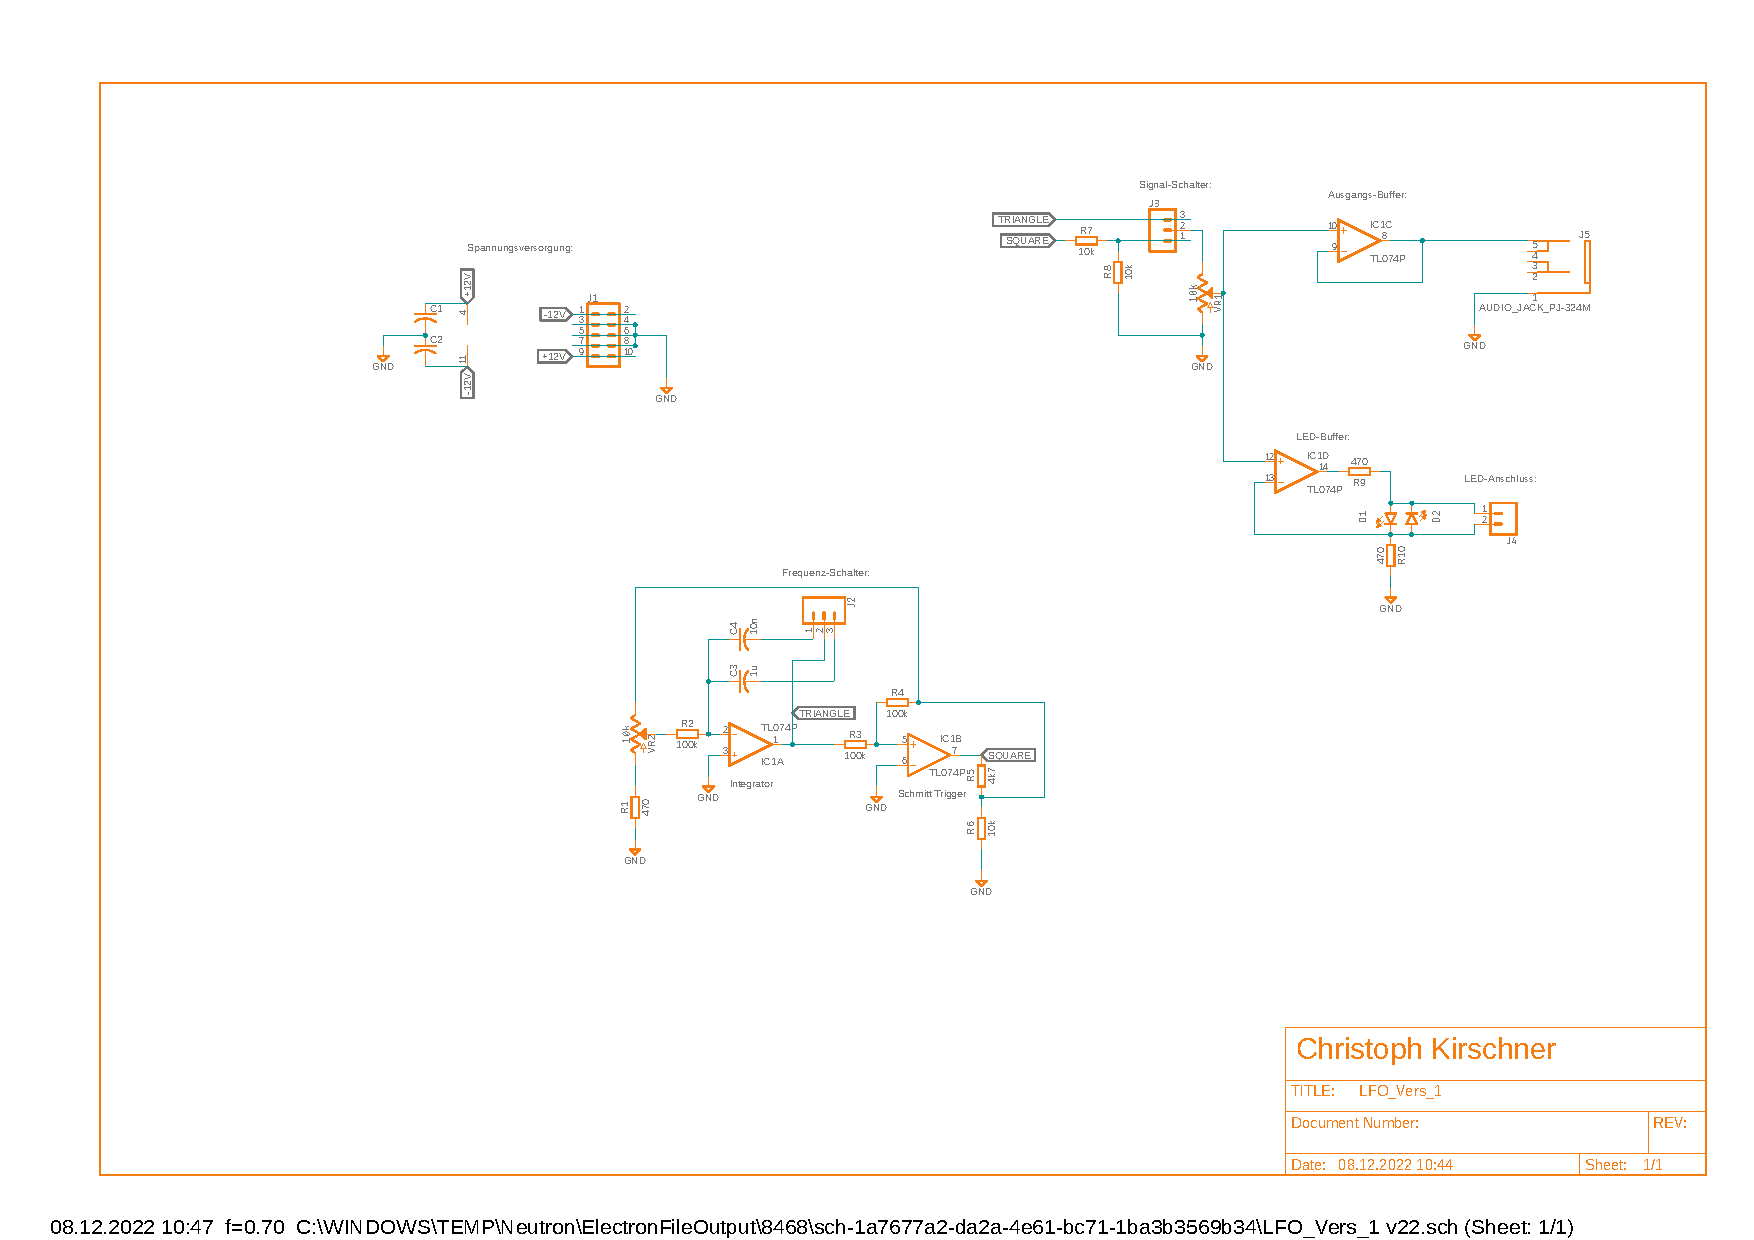
\includepdf[angle=270, clip, trim=1cm 0.8cm 0.8cm 0.8cm, scale=0.8] {figures/Schaltplan_LFO_Kirschner_08_12_22.pdf}
\caption{Fusion360 Schaltplan des LFO}
\label{fig:LFO_Stromlaufplan}
\end{figure}
 
\newpage

\section{Platine}
bla bla bla

\section{Mechanischer Aufbau}
bla bla bla